\documentclass{article}
\usepackage[margin=1in]{geometry}
\usepackage{../common}
\usepackage{../pagesetup}
\usepackage{tikz}
\newcommand{\pa}{\text{pa}}
\newcommand{\ch}{\text{ch}}
\newcommand{\bel}{\text{bel}}
\newcommand{\m}{\text{m}}
\newcommand{\nbr}{\text{nbr}}
\begin{document}

\lecture{11}{October 11}{Sasha Rush}{Ismail Ben Atitallah, Hao Wu, Raphael Rovinov, Ziliang Che, Jiaoyang Huang}{Exact Inference: Belief Propagation}

\section{Simple Marchov Chain}
For a simple Markov Chain with time limit $T$ and $V$ classes per node:
\begin{align*}
p(y,t) &=\exp(\sum_{t}\theta_t^T(y_{t-1},y_t) + \theta_t^o(y_t)-A(\theta))\\
&\propto \prod_{t} \psi_t(y_{t-1},y_t) \psi_t(y_t)
\end{align*}
\begin{center}
\begin{tikzpicture}
  %Define nodes
  \node[latent]  (y1) {$y_1$};
  \node[latent, right=of y1] (y2) {$y_2$};
  \node[latent, right=of y2] (y3) {$y_3$};
  
  \node[latent,draw=none, right=of y3] (yd) {\dots};
  \node[latent, right=of yd] (yS) {$y_S$};
  \node[latent, draw=none,right=of yS] (ydd) {\dots};
  \node[latent, right=of ydd] (yT) {$y_T$};
  
\path
	(y1) edge (y2)
	(y2) edge (y3)
	(y3) edge (yd)
	(yd) edge (yS)
	(yS) edge (ydd)
	(ydd) edge (yT);
\end{tikzpicture}
\end{center}

\subsection{Distributive Property}
Marginal:
\begin{align*}
p(y_s=v) &= \sum_{y_{1:T,y_s' =v}}\prod_{t}\psi_t(y_{t-1}',y_t')\psi(y_t')/Z(\theta)\\
&=\sum_{y_t'}\psi_T(y_T')\sum_{y_T-1}'\psi_{T-1}(y_{t-1}')\psi_T(y_{T-1},y_T') \sum \ldots \sum_{y_2'} \psi_2(y_2')\sum_{y_1'}\psi_1(y_1',y_2')\psi_1(y_1')
\end{align*}
\subsection{Compute All Marginals with Dynamic Programming}
\begin{align*}
\bel_t^-(y_t) &\propto \psi_t(y_t) \m_{t-1 \rightarrow t}^-(y_t)\\
\m_{t-1\rightarrow t}^- &=\sum_{y_{t-1}}\psi_{t-1}(y_{t-1},y_t)\bel_{t-1}^-(y_{t-1})\\
\m_{t+1\rightarrow t}^+ &= \sum_{y_{t+1}}\psi_{t+1}(y_{t+1},y_t)\psi_{t+1}(y_{t+1})\m_{t+2\rightarrow t+1}^+(y_{t+1})\\
p(y_t)&=\bel_t(y_t)\propto \m_{t+1\rightarrow t}(y_t)\bel_t^-(y_t)
\end{align*}
\begin{center}
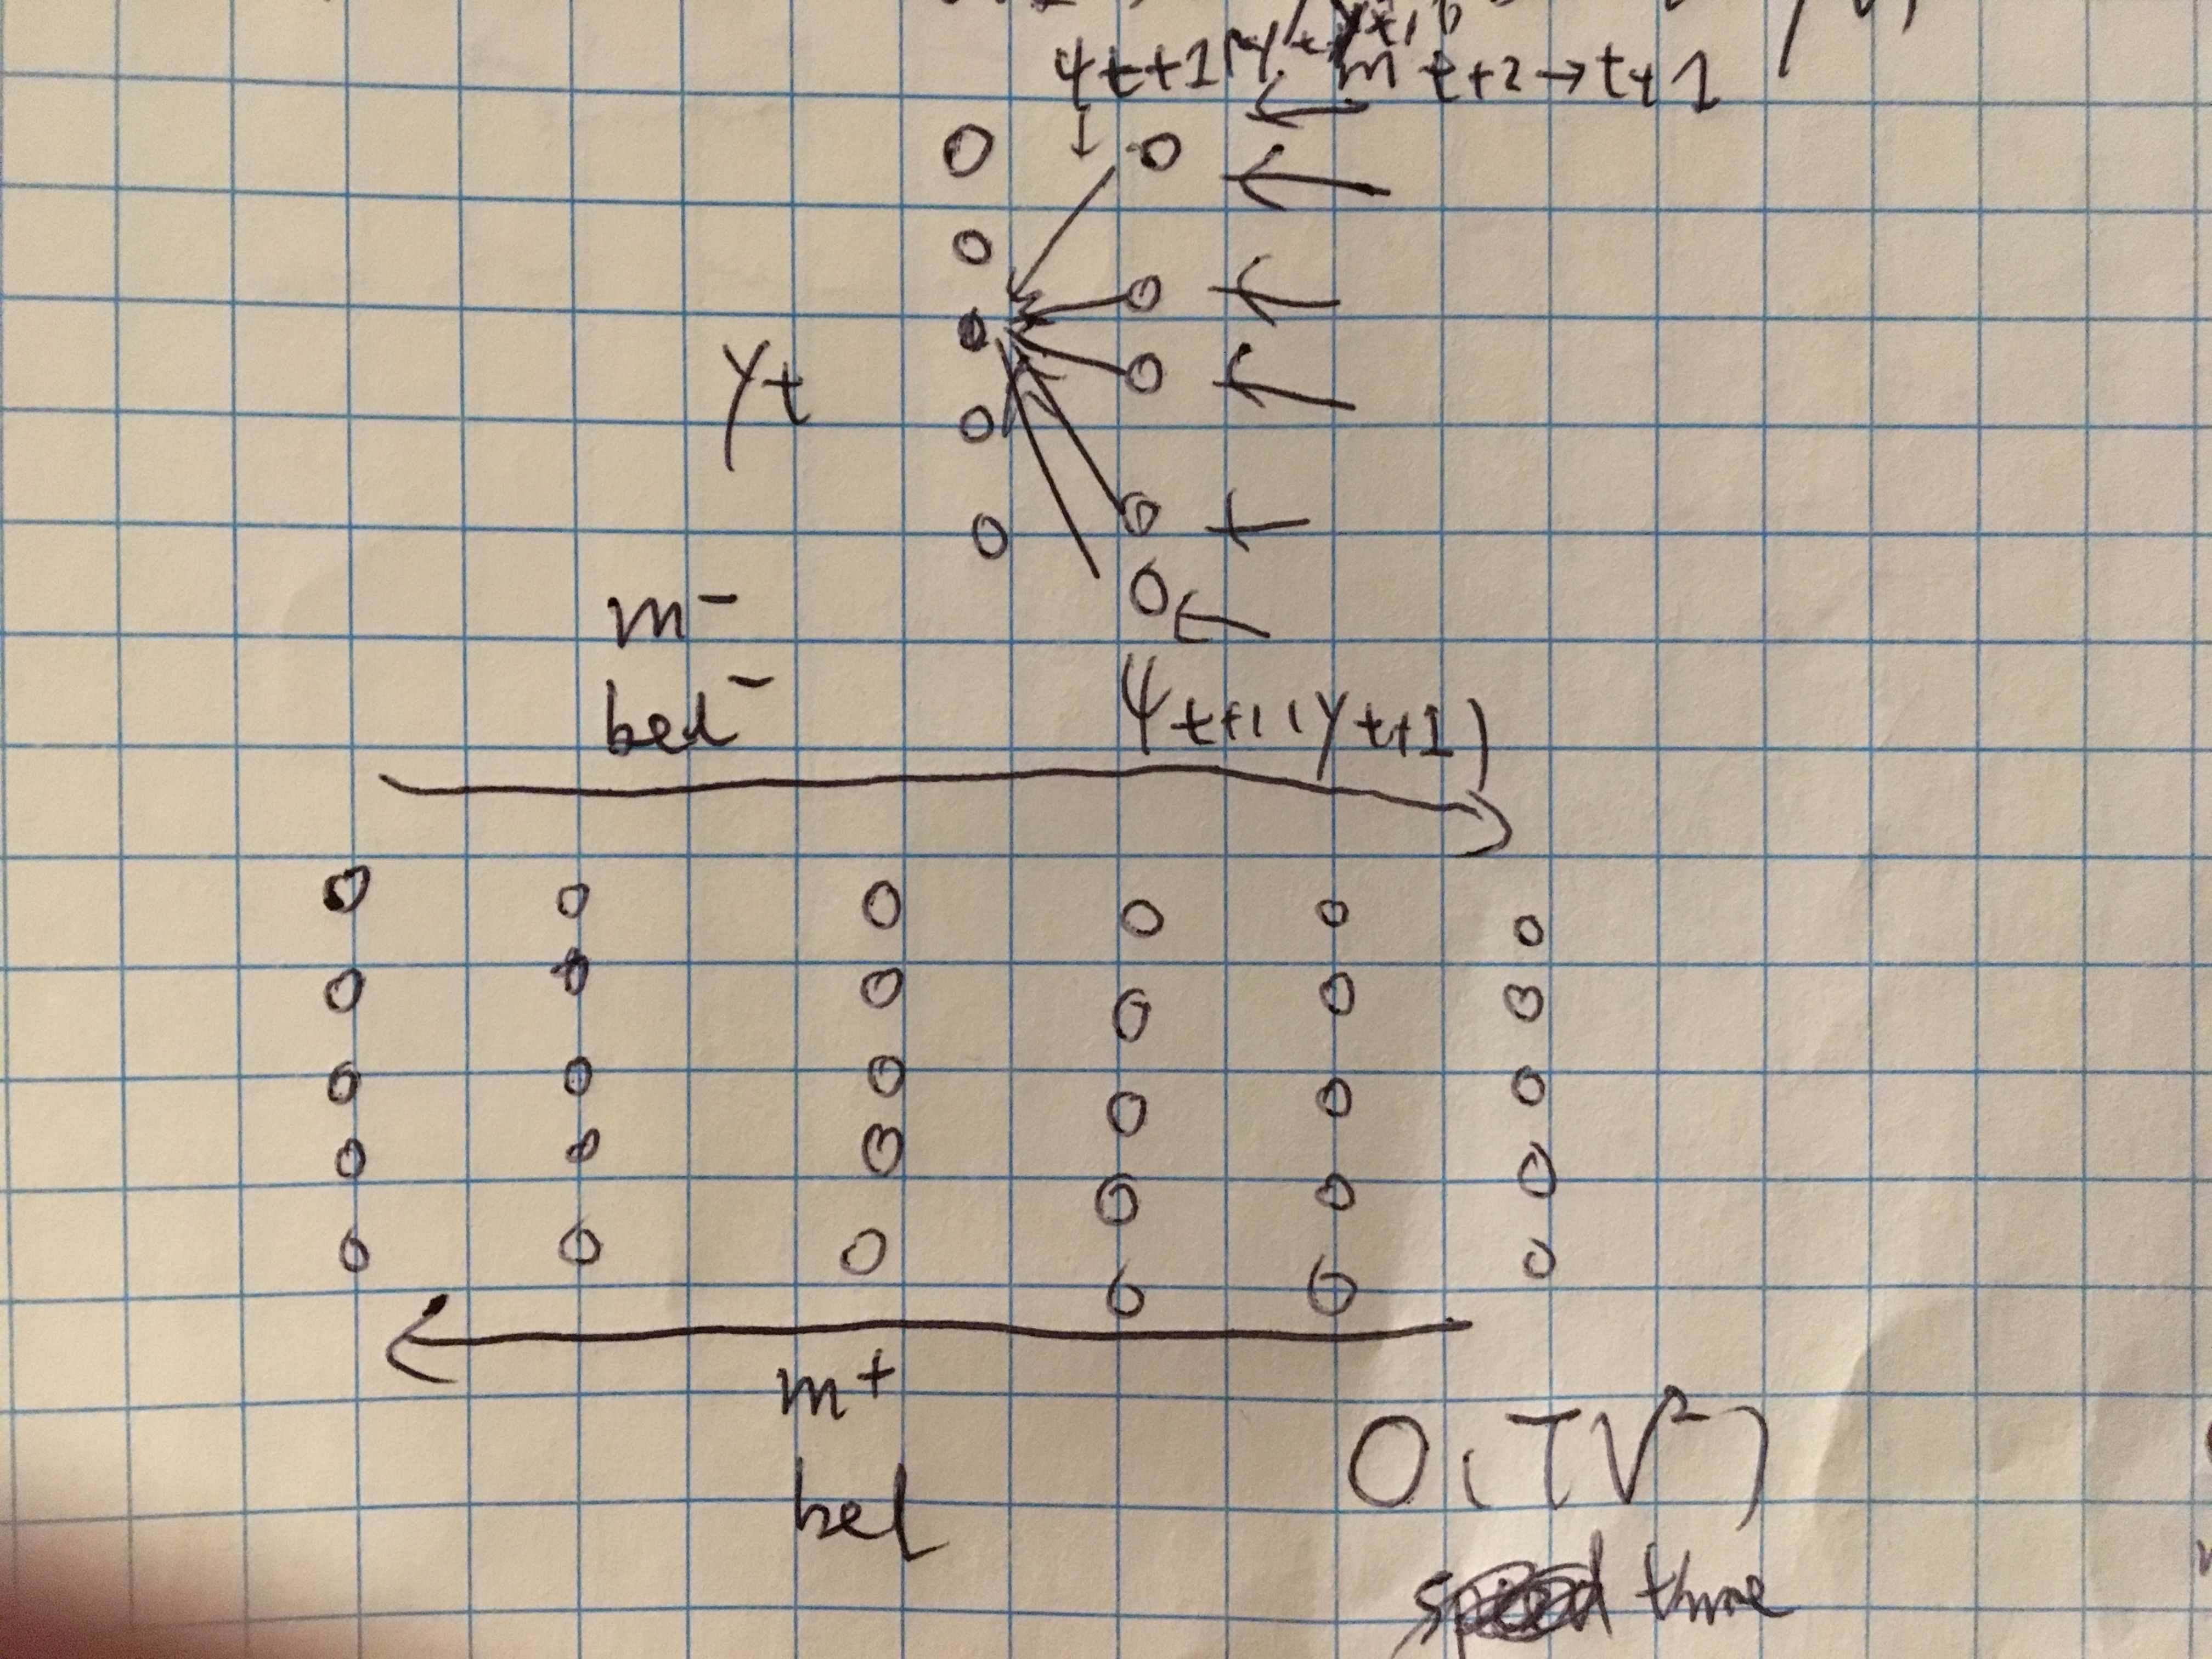
\includegraphics[scale=0.1]{g1.jpg}
\end{center}
\section{Other Graphs}
\begin{align*}
p(y_s = v) = \sum_{y',y'_s=v}\prod_c\psi_c(y_c')
\end{align*}
\begin{center}
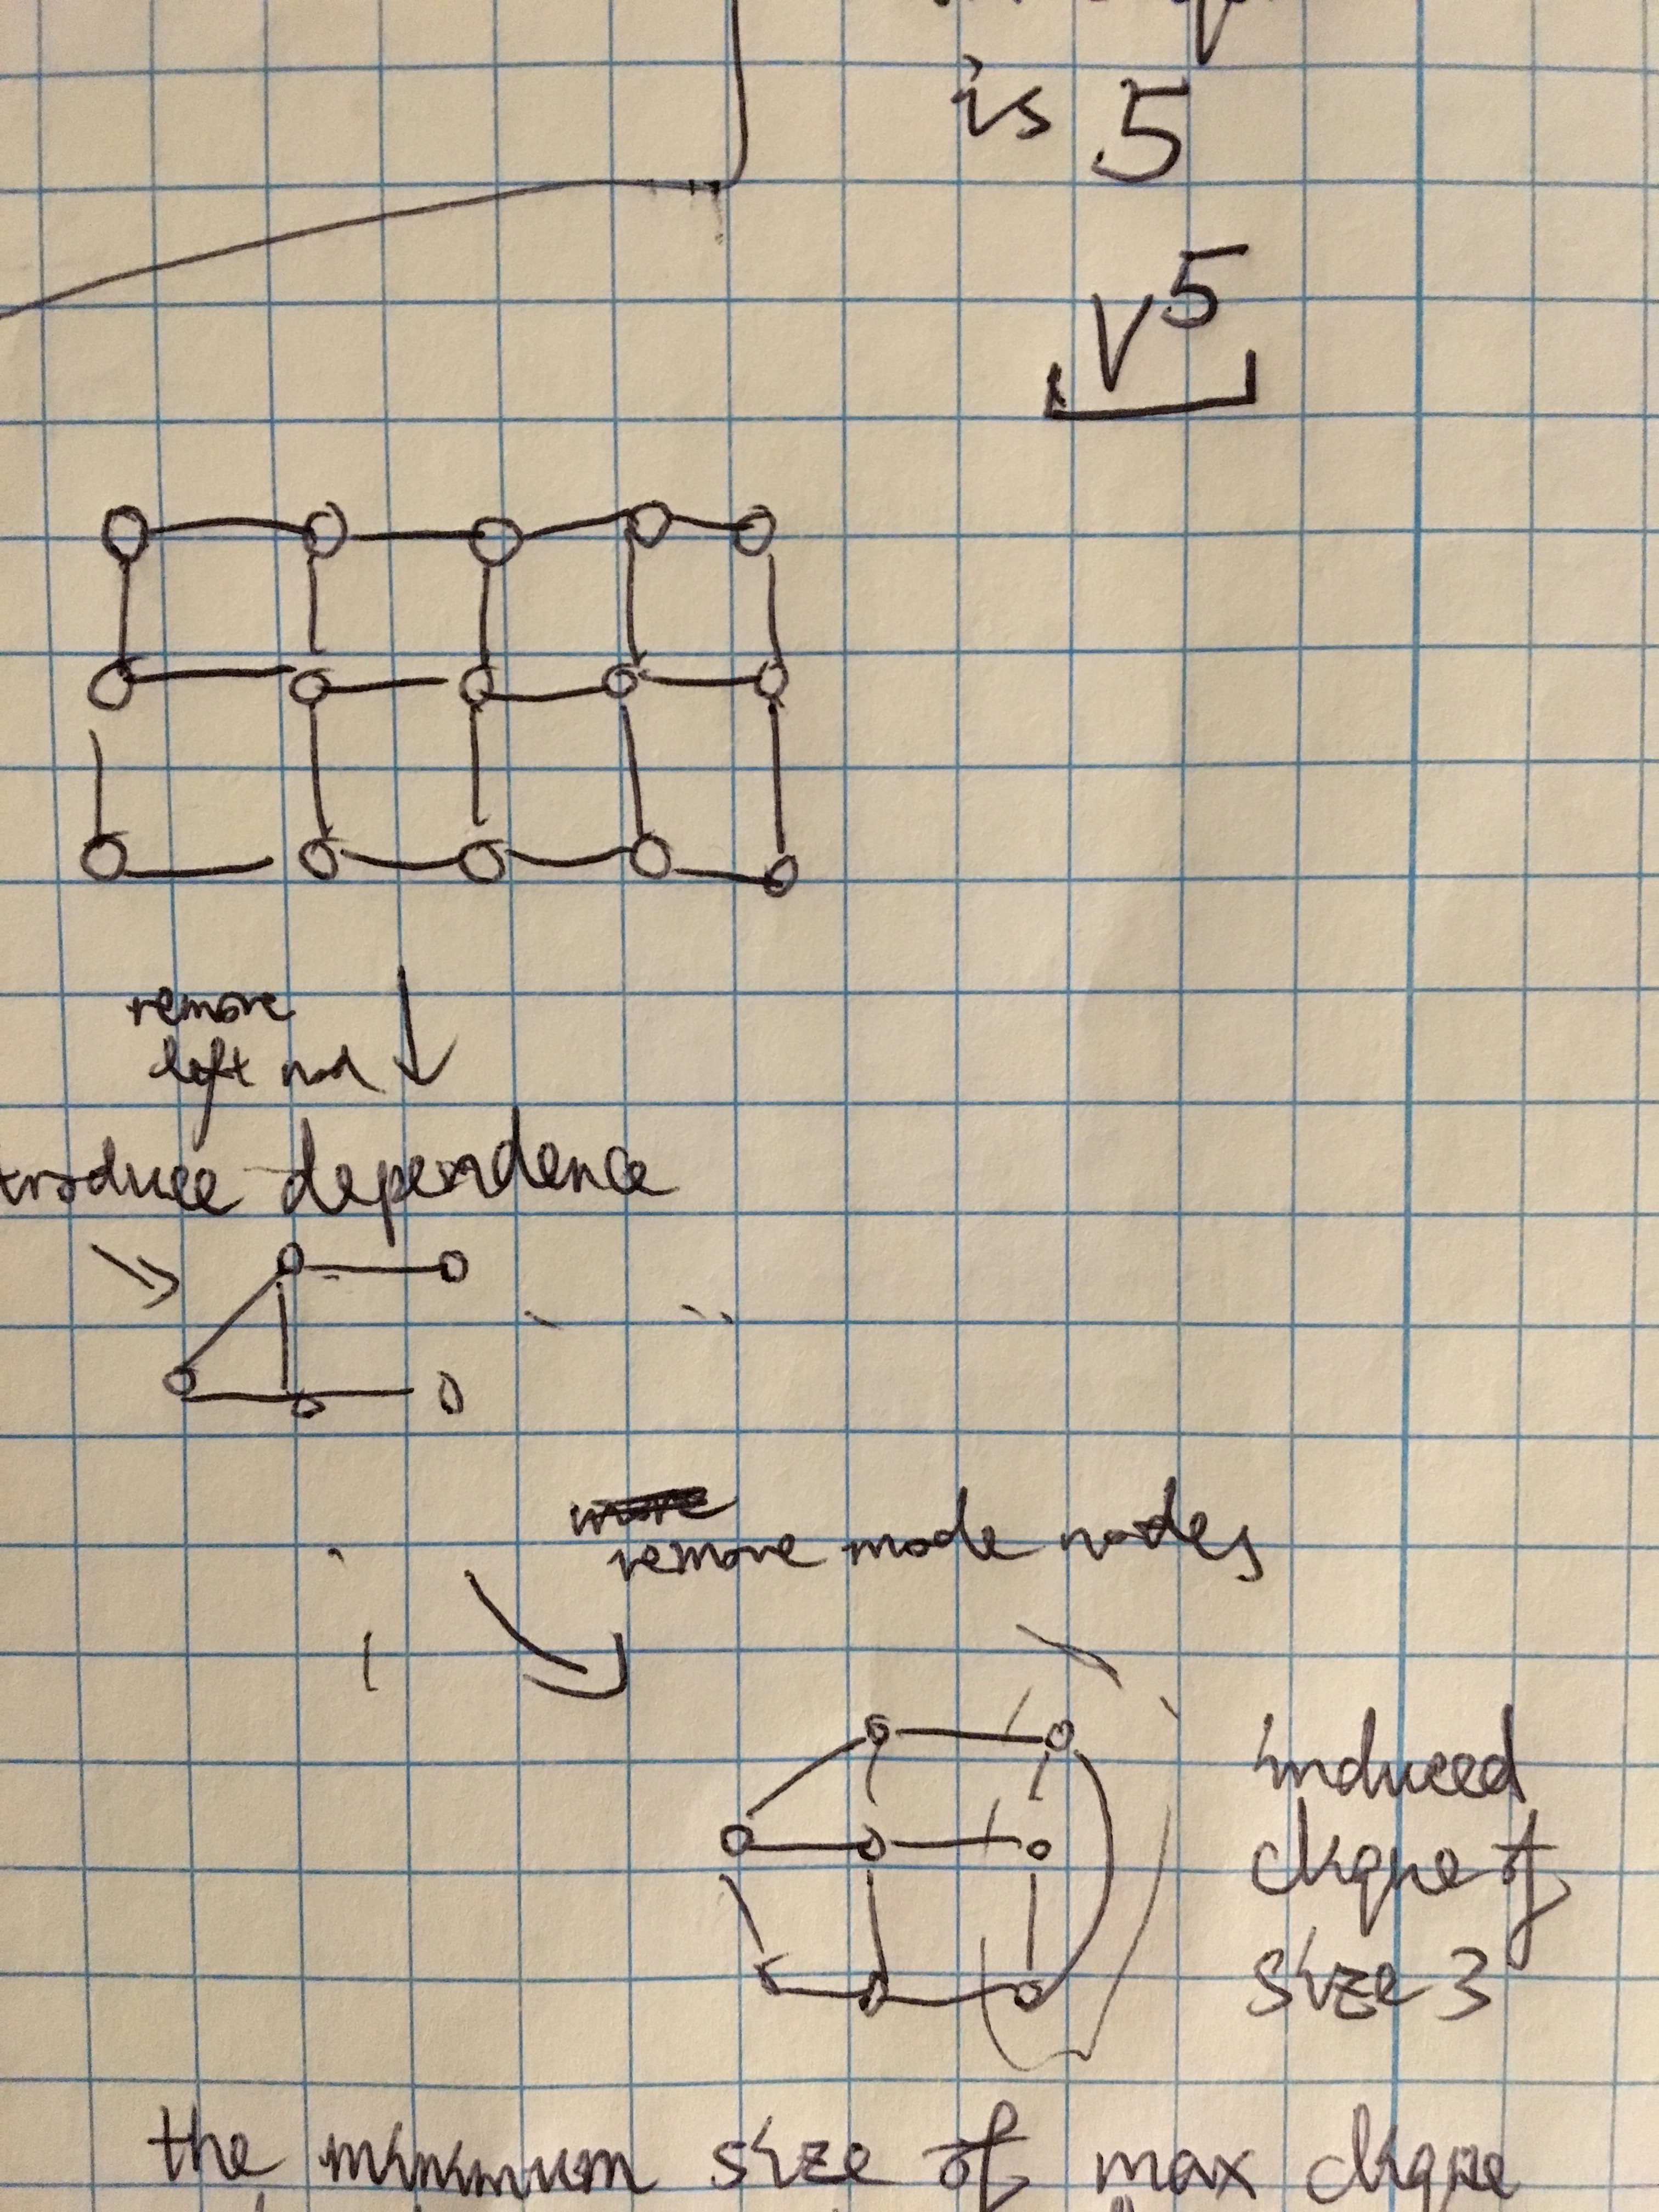
\includegraphics[scale=0.1]{g3.jpg}
\end{center}
Computing this sum product might be hard. Here we define the minimum size of maximum clique indcued -1 to be the \textit{treewidth} of the graph.
\subsection{Compute Marginals for treewidh = 1 Graph}
\begin{center}
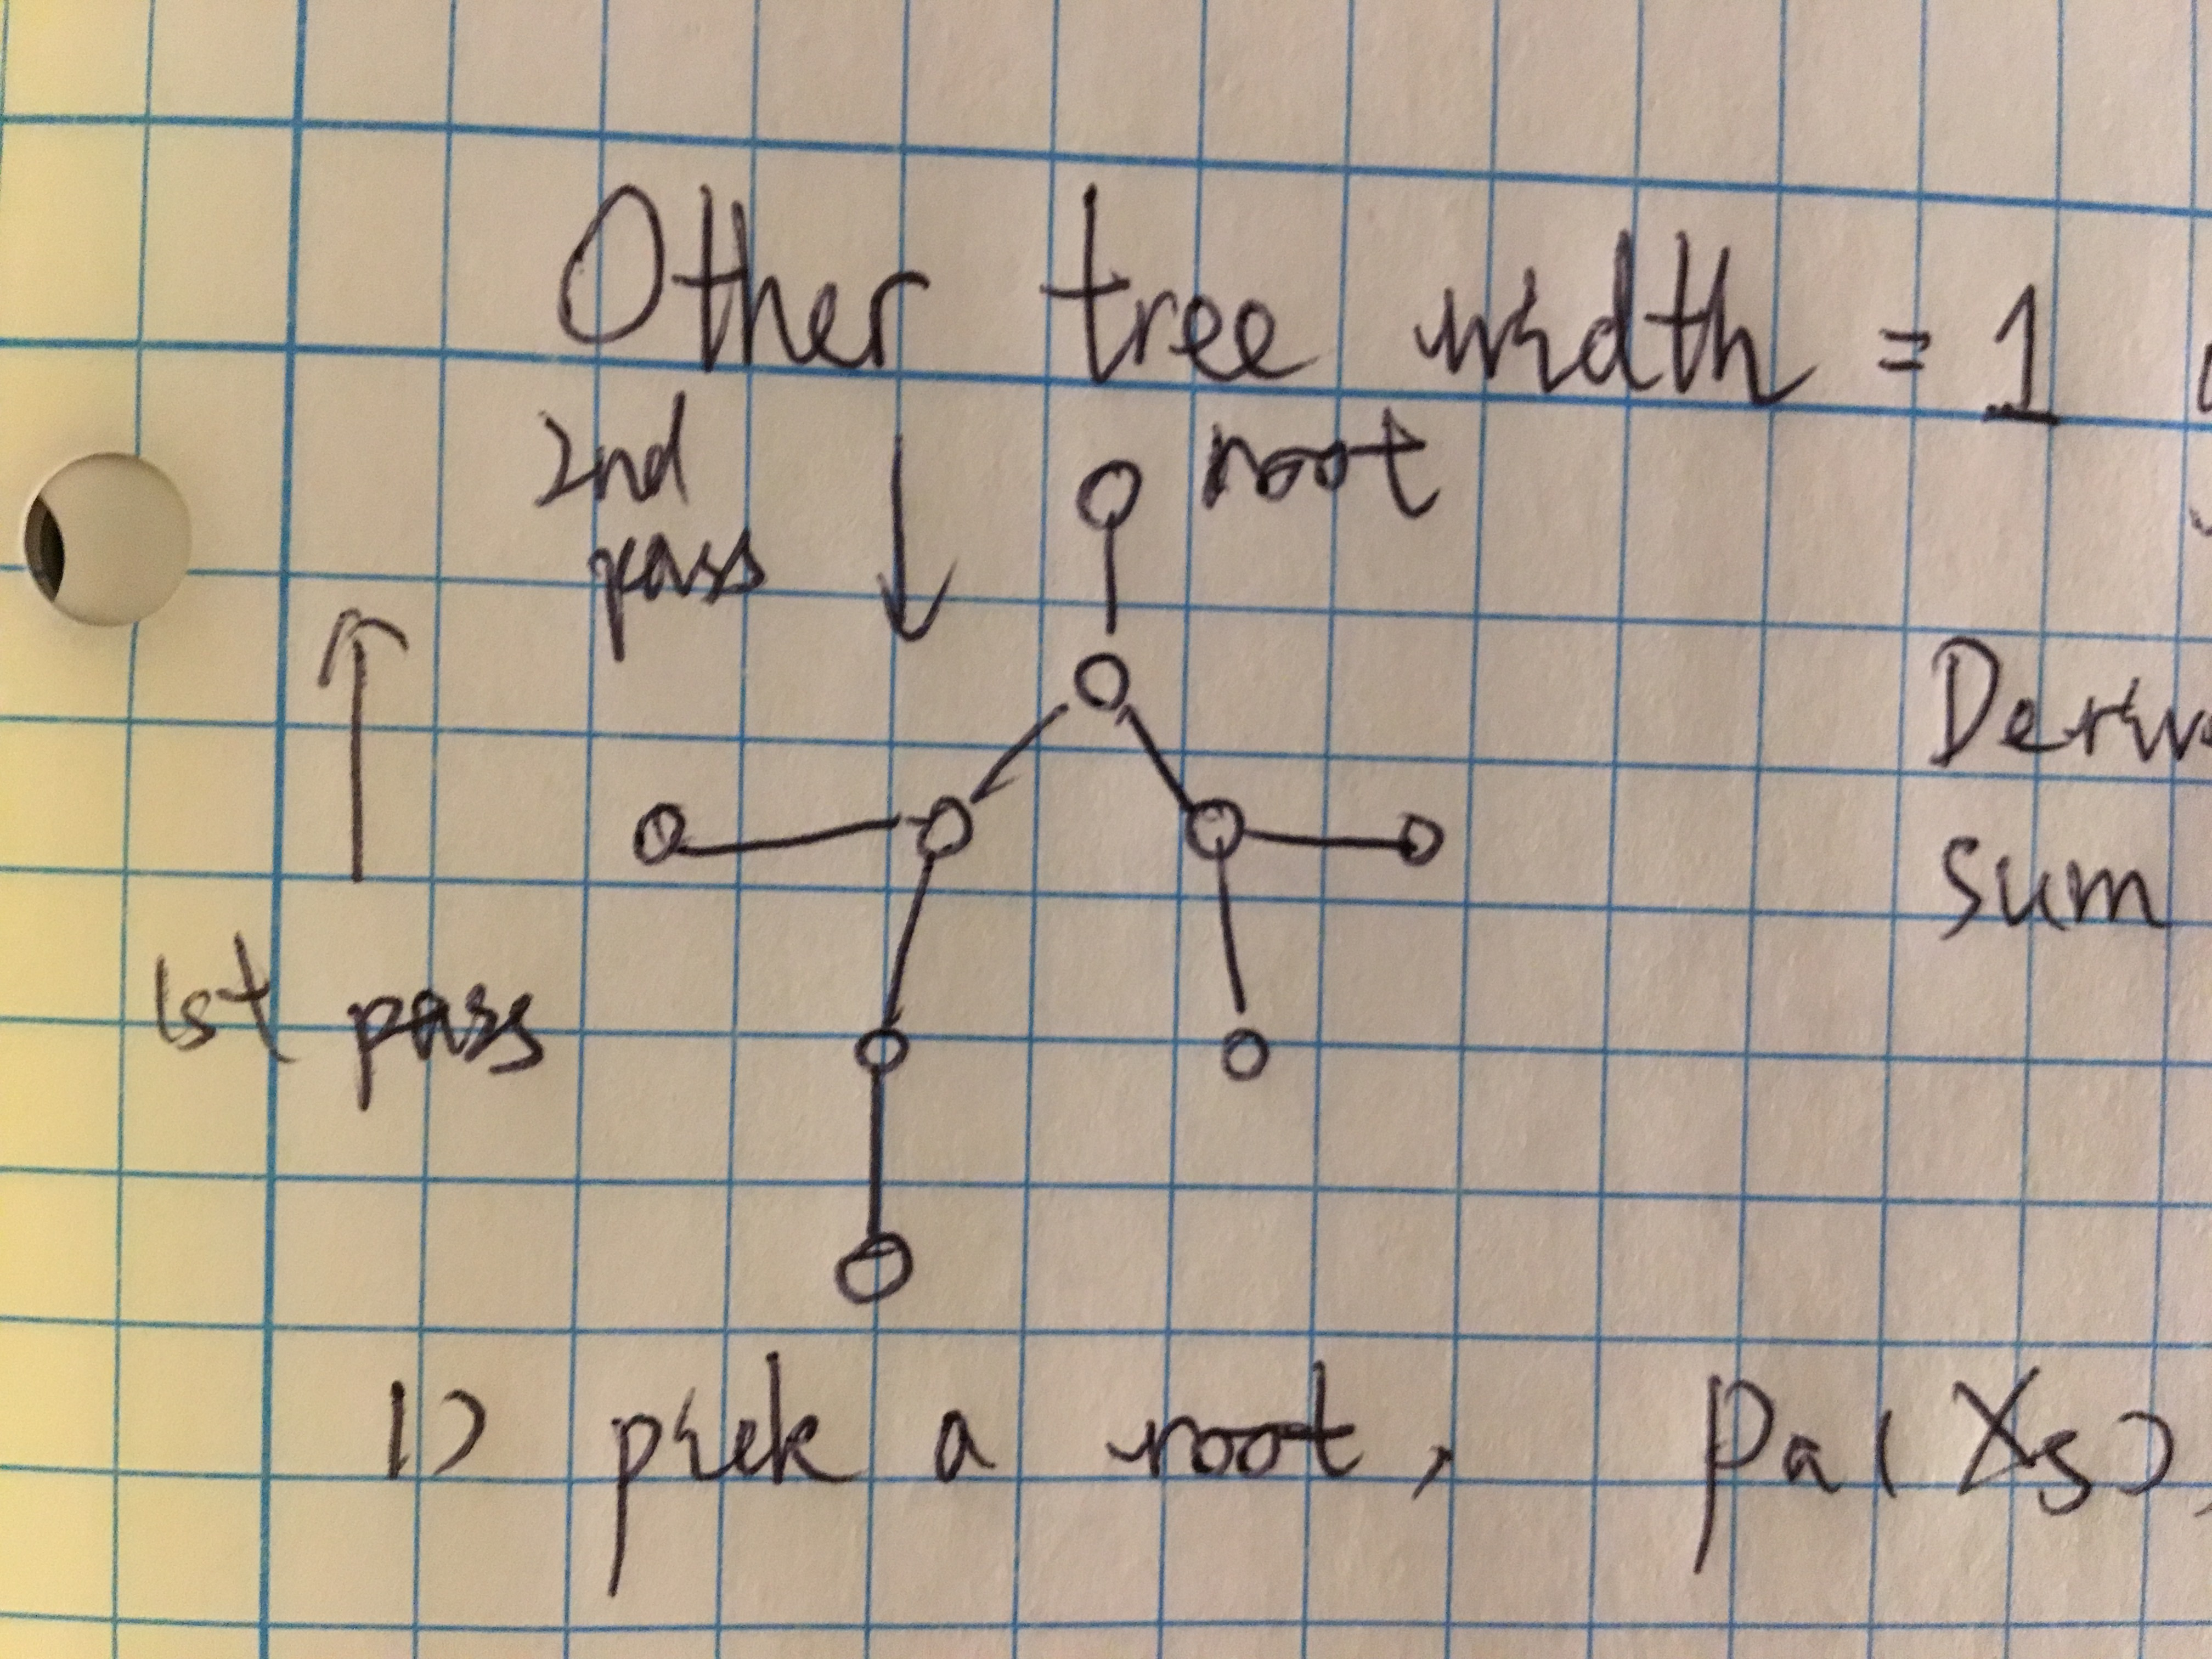
\includegraphics[scale=0.1]{g2.jpg}
\end{center}
Here we derive the generalization of the forward-backward sum-product algorithm
\begin{enumerate}
\item Pick a root  $s$, $\pa(x_s)$,$\ch(x_s)$
\item Upward pass:
\begin{align*}
\m_{s\rightarrow t}(x_t)&=\sum_{x_s}\psi_{s-t}(x_s,x_t)\bel_s^-(x_s)\\
\bel_t^-(x_t)&\propto \psi_t(x_t)\prod_{s \in \ch(t)} m_{s-t}^-(x_t)
\end{align*}
\item Downward pass:
\begin{align*}
\bel_s(x_s)&\propto \bel_s^-(x_s)\prod_{t \in \pa(s)} \m_{t\rightarrow s}^+(x_s) \\
\m_{t\rightarrow s}^+ (x_s) &= \sum_{x_t} \psi{s-t}(x_s,x_t)\psi_t(x_t)\prod_{c \in \ch(t), c \neq s}=\m_t^-(x_t)
\end{align*}
\end{enumerate}

\section{Parallel Protocol for Sum Product}

\begin{align*}
\bel_s(x_s)&\propto\psi_s(x_s)\prod_{t \in \nbr(s)} \m_{t\rightarrow s}(x_s)\\
\m_(s\rightarrow t) &=\sum_{x_s}\psi_s(x_s)\psi_{s-t}\prod_{u \in \nbr(s), u \neq t}(x_s)
\end{align*}
\section{Final Notes}
For this lecture we have been ultilizing + and $\times$ and distributive property
\subsection{Commutative Semi-ring}
\begin{center}
\begin{tabular}{ c c c }
$+$ & max & $\cap$\\ 
 $\times$ & $\times$& $\cup$ \\  
 $ \vee$&  $ \vee$&  $\vee$\\
 marginal & argmax & satisfying assignment    
\end{tabular}
\end{center}
\end{document}

